% \levelC{Hardware}
The experiments did not take advantage of GPU acceleration and were  conducted on a single computer with 256GB of RAM and with 2 Intel\textregistered Xeon\textregistered E5-2630 v2 processors, with 6 cores each, with 2 hyper-threads per core, or 24 hyper-threads in total. 


% \levelC{Software}
The main software and frameworks used to build the experiments were Python 3.6 
\cite{rossum_python_2019}, Jupyter notebook \cite{perez_jupyter_2019}, Tensorflow 1.14.0 \cite{google_brain_tensorflow_2019}, Keras 2.2.4-tf \cite{chollet_keras_2019}, and Fedora Linux 27.
% repository
The source code for the experiments is available at \sloppy\url{http://github.com/atilaromero/carving-experiments}.


\begin{table}[!ht]
    \centering
    \caption[Complement of entropy measure]{Complement of entropy measure.}
    \label{tab:pass1}
\begin{tabular}{|l|l|l|l|l|l|l|}
\hline
Category & GovdocsACC & RandomACC & Time   & Epochs & GovdocsTP & GovdocsPrec \\ \hline
dwf      & 0.528           & 0.914          & 16m16s & 37     & 0.483589  & 0.915888         \\ \hline
gz       & 0.613           & 0.906          & 16m59s & 37     & 0.572848  & 0.934499         \\ \hline
swf      & 0.592           & 0.970          & 19m58s & 43     & 0.579381  & 0.978685         \\ \hline
kmz      & 0.589           & 0.983          & 16m21s & 36     & 0.581892  & 0.987932         \\ \hline
png      & 0.659           & 0.960          & 19m40s & 46     & 0.644792  & 0.978440         \\ \hline
pdf      & 0.674           & 0.977          & 29m59s & 70     & 0.666325  & 0.988613         \\ \hline
pps      & 0.748           & 0.962          & 26m12s & 57     & 0.738046  & 0.986692         \\ \hline
pptx     & 0.827           & 0.828          & 12m59s & 30     & 0.791063  & 0.956545         \\ \hline
ppt      & 0.827           & 0.977          & 28m18s & 63     & 0.822927  & 0.995075         \\ \hline
gif      & 0.848           & 0.991          & 16m40s & 39     & 0.846620  & 0.998372         \\ \hline
jpg      & 0.865           & 0.990          & 25m31s & 59     & 0.863636  & 0.998424         \\ \hline
doc      & 0.885           & 0.990          & 14m13s & 31     & 0.883838  & 0.998687         \\ \hline
eps      & 0.989           & 1.000          & 8m00s  & 19     & 0.989000  & 1.000000         \\ \hline
ps       & 0.990           & 1.000          & 4m55s  & 11     & 0.990000  & 1.000000         \\ \hline
xls      & 0.991           & 1.000          & 9m51s  & 23     & 0.991000  & 1.000000         \\ \hline
sql      & 0.995           & 1.000          & 5m19s  & 11     & 0.995000  & 1.000000         \\ \hline
kml      & 0.995           & 1.000          & 7m43s  & 16     & 0.995000  & 1.000000         \\ \hline
log      & 0.998           & 1.000          & 5m19s  & 12     & 0.998000  & 1.000000         \\ \hline
wp       & 0.998           & 1.000          & 5m19s  & 11     & 0.998000  & 1.000000         \\ \hline
hlp      & 1.000           & 1.000          & 4m49s  & 11     & 1.000000  & 1.000000         \\ \hline
rtf      & 1.000           & 1.000          & 5m17s  & 12     & 1.000000  & 1.000000         \\ \hline
html     & 1.000           & 1.000          & 5m01s  & 11     & 1.000000  & 1.000000         \\ \hline
f        & 1.000           & 1.000          & 4m50s  & 11     & 1.000000  & 1.000000         \\ \hline
java     & 1.000           & 1.000          & 5m18s  & 11     & 1.000000  & 1.000000         \\ \hline
txt      & 1.000           & 1.000          & 4m42s  & 11     & 1.000000  & 1.000000         \\ \hline
csv      & 1.000           & 1.000          & 5m19s  & 12     & 1.000000  & 1.000000         \\ \hline
xml      & 1.000           & 1.000          & 5m14s  & 11     & 1.000000  & 1.000000         \\ \hline
dbase3   & 1.000           & 1.000          & 4m42s  & 11     & 1.000000  & 1.000000         \\ \hline
\end{tabular}
\end{table}

The results obtained are shown in Table \ref{tab:pass1}. The entropy measure is the complement of the GovdocsTP column.  The GovdocsACC columns contains the accuracy validations values as calculated by Keras on the Govdocs1 dataset, thus considering all samples labeled as ``random'' as errors. The RandomACC column lists the portion of samples from the random generator classified as ``random'' by the model for that file type. The Time and Epoch columns refer to the training session of each model. The GovdocsTP column uses the equation \ref{eq:TPend}, giving the complement of the entropy. GovdocsPrec is simply $GovdocsTP/GovdocsACC$.

Figure \ref{fig:not_random} shows, for each file type, the percent of 512-byte fragments identified as ``structured'', from a sample of 1000 fragments for each file type.
In the figure, the 87\% value for JPG, for example, means that up to 87\% of the blocks of the JPG dataset have recognizable patterns. Since the assumption of no false negatives was used, the real value, which is unknown, can be lower. The entropy measure proposed is the complement of this value, for example, 13\% for JPG.

\noindent
\begin{figure*}[htb!]
\centering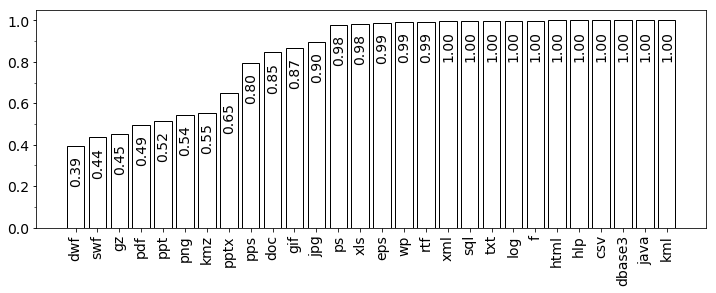
\includegraphics[width=1.0\textwidth]{content/random.png}
\caption[Complement of entropy measure for 28 file types]{\label{fig:not_random}Estimate of the percentage of samples with recognizable structures, using models trained to distinguish each file type from random data. }%
\end{figure*}
